\documentclass[dvipsnames,hidelinks,t]{beamer}

  % Enables the use of colour.
  \usepackage{xcolor}
  % Syntax high-lighting for code. Requires Python's pygments.
  \usepackage{minted}
  % Enables the use of umlauts and other accents.
  \usepackage[utf8]{inputenc}
  % Diagrams.
  \usepackage{tikz}
  % Settings for captions, such as sideways captions.
  \usepackage{caption}
  % Symbols for units, like degrees and ohms.
  \usepackage{gensymb}
  % Latin modern fonts - better looking than the defaults.
  \usepackage{lmodern}
  % Allows for columns spanning multiple rows in tables.
  \usepackage{multirow}
  % Better looking tables, including nicer borders.
  \usepackage{booktabs}
  % More math symbols.
  \usepackage{amssymb}
  % More math fonts, like mathbb.
  \usepackage{amsfonts}
  % More math layouts, equation arrays, etc.
  \usepackage{amsmath}
  % More theorem environments.
  \usepackage{amsthm}
  % More column formats for tables.
  \usepackage{array}
  % Adjust the sizes of box environments.
  \usepackage{adjustbox}
  % Better looking single quotes in verbatim and minted environments.
  \usepackage{upquote}
  % Better blank space decisions.
  \usepackage{xspace}
  % Better looking tikz trees.
  \usepackage{forest}
  % URLs.
  \usepackage{hyperref}
  % For plotting.
  \usepackage{pgfplots}
  
  % Various tikz libraries.
  % For drawing mind maps.
  \usetikzlibrary{mindmap}
  % For adding shadows.
  \usetikzlibrary{shadows}
  % Extra arrows tips.
  \usetikzlibrary{arrows.meta}
  % Old arrows.
  \usetikzlibrary{arrows}
  % Automata.
  \usetikzlibrary{automata}
  % For more positioning options.
  \usetikzlibrary{positioning}
  % Creating chains of nodes on a line.
  \usetikzlibrary{chains}
  % Fitting node to contain set of coordinates.
  \usetikzlibrary{fit}
  % Extra shapes for drawing.
  \usetikzlibrary{shapes}
  % For markings on paths.
  \usetikzlibrary{decorations.markings}
  % For advanced calculations.
  \usetikzlibrary{calc}
  
  % GMIT colours.
  \definecolor{gmitblue}{RGB}{20,134,225}
  \definecolor{gmitred}{RGB}{220,20,60}
  \definecolor{gmitgrey}{RGB}{67,67,67}
  
  % Change some style options.
  \usetheme{metropolis}
  % Tell minted to use the following colour scheme. 
  \usemintedstyle{manni}
  % Remove some of the vertical space after the title.
  % \addtobeamertemplate{frametitle}{}{\vspace{-3mm}}
  % Change the default theme colours.
  \setbeamercolor{normal text}{fg=darkgray, bg=white}
  \setbeamercolor{alerted text}{fg=gmitred, bg=white}
  \setbeamercolor{example text}{fg=gmitblue, bg=white}
  \setbeamercolor{frametitle}{fg=gmitblue, bg=white}
  \setbeamercolor*{item}{fg=gmitblue}
  % Use a better math mode font.
  \usefonttheme[onlymath]{serif}
  % Don't display section pages.
  \metroset{sectionpage=none}
  % Change the default itemize bullets.
  \setbeamertemplate{itemize item}{\color{gray}--}
  % Change the position of left aligned math.
  %\setlength{\mathindent}{7mm}

  % An environment for displaying math in red, without lots of vertical space.
  \newcommand{\redmath}[1]{\vspace{-3mm} {\begin{center} \color{gmitred} $ #1 $ \end{center}} \vspace{-2mm}}

  % For displaying a blank character.
  \newcommand{\bl}{\underline{\hspace{2mm}}}

  % \citeurl can be used to a clickable short url to a slide as a reference.
  \renewcommand\footnoterule{}
  \newcommand{\citeurl}[1]{\let\thefootnote\relax\footnotetext{\tiny \textcolor{gmitgrey}{\href{http://#1}{#1}}}}
  \newcommand{\citeeg}[1]{\let\thefootnote\relax\footnotetext{\tiny \textcolor{gmitgrey}{#1}}}
  
  % Prevent minted from showing errors.
  \makeatletter
  \expandafter\def\csname PYGdefault@tok@err\endcsname{\def\PYGdefault@bc##1{{\strut ##1}}}
  \makeatother
  
  \begin{document}
    \title{Computational complexity}
    \subtitle{}
    \author{ian.mcloughlin@gmit.ie}
    \date{}
  
    \begin{frame}
      \titlepage
    \end{frame}
  
    \begin{frame}{Computational complexity}
  \begin{description}
    \setlength\itemsep{6mm}
    \item[Length] of the input ($n$).
    \item[Number] of lookups of the Turing machine state table.
    \item[Function:] number of lookups versus length of input.
    \item[Worst case] only.
  \end{description}
  \redmath{f(n) = n \log{n}}
\end{frame}


\begin{frame}{Average vs. worst case}
  \begin{table}
    \begin{tabular}{p{2cm}rr}
      Input & Algorithm A & \hspace{1cm} Algorithm B \\
      \hline
      (1,2,3) &  1ms &  1ms \\
      (1,3,2) &  1ms &  5ms \\
      (2,1,3) &  2ms &  4ms \\
      (2,3,1) &  2ms &  5ms \\
      (3,1,2) &  2ms &  5ms \\
      (3,2,1) & 10ms &  4ms \\
      \hline
      Average &  3ms &  4ms \\
      Worst   & 10ms &  5ms
    \end{tabular}
  \end{table}
  \begin{center}
    Would you choose Algorithm A or Algorithm B?
  \end{center}
\end{frame}


\begin{frame}[fragile]{Terminology of complexity (graph)}
  \begin{center}
    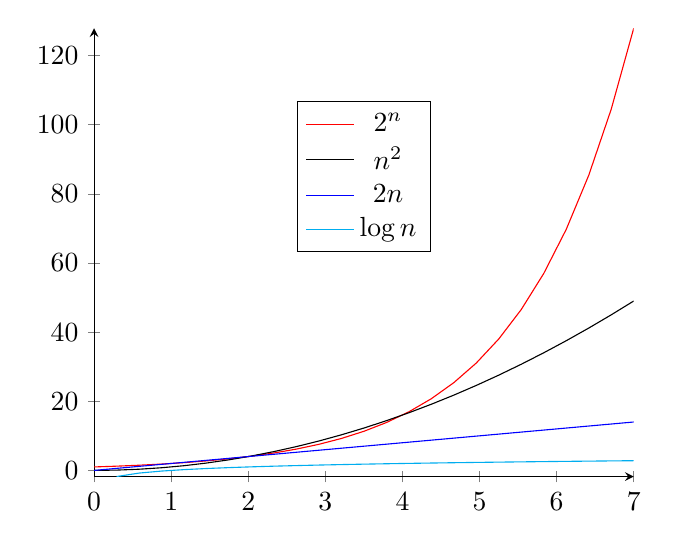
\begin{tikzpicture}
      \begin{axis}[xmin=0, domain=0:7, axis x line=bottom, axis y line=left, legend style={at={(0.5,0.5)},anchor=south}]
        \addplot[red]   {pow(2,x)};
        \addplot[black] {pow(x,2)};
        \addplot[blue]  {2*x};
        \addplot[cyan]  {ln(x)/ln(2))};
        \legend{$2^n$,$n^2$,$2n$,$\log n$};
      \end{axis}
    \end{tikzpicture}
  \end{center}
\end{frame}
  
  
\begin{frame}{Linear}
  \redmath{f(n) = a_0 + a_1 n}
  \begin{exampleblock}{How many pairs of shoes does a centipede need?}
    \begin{itemize}
      \item Let's say a centipede has 100 feet.
      \item Then every centipede needs 100 shoes.
      \item That's 50 pairs of shoes.
      \item So 2 centipedes need 100 pairs, 3 need 150 pairs, etc.
      \item So $n$ centipedes need $50n$ pairs of shoes.
      \item Linearity is familiar, and most people's default assumption.
      \item You take the input, multiply by a constant, and add another constant.
    \end{itemize}
  \end{exampleblock}
\end{frame}
  
  
\begin{frame}{Polynomial}
  \redmath{f(n) = a_0 + a_1 n + a_2 n^2 + a_3 n^3 + \ldots}
  \begin{exampleblock}{What is the volume of a cube of side $n$?}
    \begin{itemize}
      \item Suppose we have a cube with sides of length 1 metre.
      \item The volume of the cube is $1 \times 1 \times 1 = 1$ metres cubed.
      \item Suppose the cube has sides of length 2 metres instead.
      \item The volume of the cube is $2 \times 2 \times 2 = 8$ metres cubed.
      \item In general, for sides of length $n$, the volume is $n^3$.
    \end{itemize}
  \end{exampleblock}
\end{frame}
  
  
\begin{frame}{Exponential}
  \redmath{f(n) = a^n}
  \begin{exampleblock}{How many numbers can we represent with $n$ bits?}
    \begin{itemize}
      \item Consider the case of four bits -- imagine four placeholders \textbf{\fbox{?}}\textbf{\fbox{?}}\textbf{\fbox{?}}\textbf{\fbox{?}}
      \item Each placeholder can contain either 0 or 1.
      \item There are $2 \times 2 \times 2 \times 2 = 2^4 = 16$ different numbers.
      \item Add another bit, how many numbers is it now?
      \item It's $2 \times 2 \times 2 \times 2 \times 2 = 2^5 = 32$.
      \item Generally $n$ bits can represent $2^n$ numbers.
    \end{itemize}
  \end{exampleblock}
\end{frame}
  
  
\begin{frame}{Logarithmic}
  \redmath{f(n) = \log_a n}
  \begin{exampleblock}{How many bits do we need to represent $n$ numbers?}
    \begin{itemize}
      \item If we have $n$ bits we can represent $2^n$ numbers.
      \item If we want to represent $n$ numbers, how many bits to we need (at a minimum)?
      \item The inverse operation to exponentiation is logarithm.
      \item Remember, $a^n = b$ means $\log_a b = n$.
    \end{itemize}
  \end{exampleblock}
\end{frame}
  
\begin{frame}{Big-O (Sipser)}
  \begin{definition}
    Let $f$ and $g$ be functions $f,g: \mathbb{N} \rightarrow \mathbb{R}^+$.
    We say that $f(n) = O(g(n))$, or $f$ is \emph{big-O} of $g$, if positive integers $c$ and $n_0$ exist such that, for every integer $n$ greater than or equal to $n_0$, $f(n) \le cg(n)$.
  \end{definition}
  \begin{exampleblock}{Example}
    Let $f$ be the function $f(n) = 5n^3 + 2n^2 + 22n + 6$.
    We'll prove that $f$ is big-O of $n^3$ ($f = O(n^3)$).
    Let $c$ be $6$ and $n_0$ be $10$.
    Is the following true, for all $n$ greater than or equal to 10, $5n^3 + 2n^2 + 22n + 6 \le 6n^3$?
    Note that as $n$ increases ($n=10,n=11,n=12,\ldots$), $f(n)$ also increases.
    Also note that $f(10) = 5426$ and $6g(10) = 6000$.
  \end{exampleblock}
  \citeurl{math.mit.edu/~sipser/book.html}
\end{frame}
  
  
\begin{frame}[fragile]{Big-O example graph}
  \begin{center}
    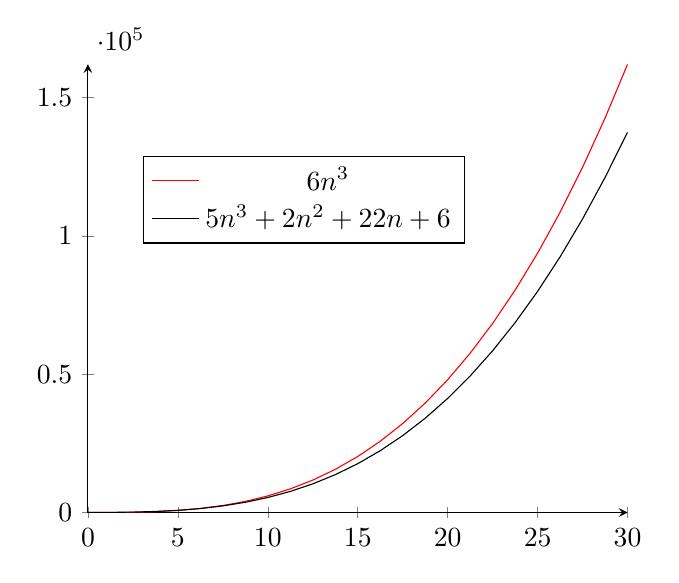
\begin{tikzpicture}
      \begin{axis}[xmin=0, domain=0:30, axis x line=bottom, axis y line=left, legend style={at={(0.4,0.6)},anchor=south}]
        \addplot[red]   {6*pow(x,3)};
        \addplot[black] {5*pow(x,3) + 2*pow(x,2) + 22*x + 6};
        \legend{$6n^3$,$5n^3 + 2n^2 + 22n + 6$};
      \end{axis}
    \end{tikzpicture}
  \end{center}
\end{frame}
  
\begin{frame}[fragile]{Smaller values of $n$}
  \begin{center}
    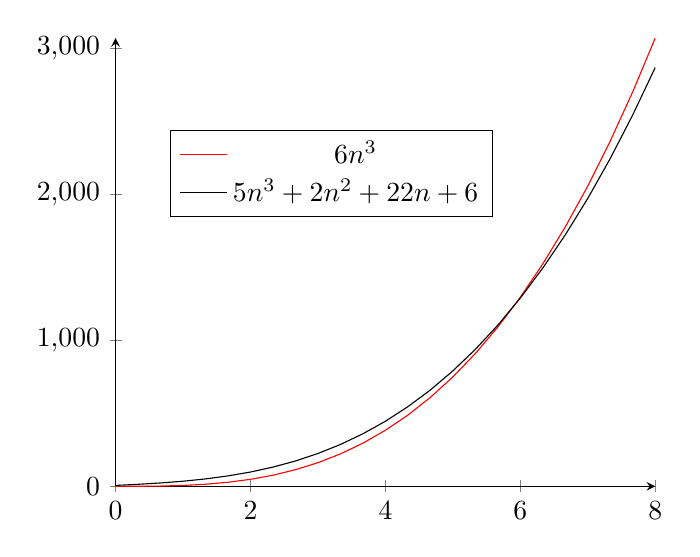
\begin{tikzpicture}
      \begin{axis}[xmin=0, domain=0:8, axis x line=bottom, axis y line=left, legend style={at={(0.4,0.6)},anchor=south}]
        \addplot[red]   {6*pow(x,3)};
        \addplot[black] {5*pow(x,3) + 2*pow(x,2) + 22*x + 6};
        \legend{$6n^3$,$5n^3 + 2n^2 + 22n + 6$};
      \end{axis}
    \end{tikzpicture}
  \end{center}
\end{frame} 
  \end{document}